\documentclass[./main.tex]{subfiles}

\begin{document}
\section{Deep Learning Theory}
The following section covers the most important background theory for the experiments in Section \ref{sec:experiments}. This includes an introduction to various types of neural networks, as well as an introduction to the optimization of such networks.

\subsection{Feedforward Neural Networks}
\textbf{Feedforward neural networks} are the most basic type of neural networks. The aim of a feedforward neural network is to approximate some function $f^*$, by defining a mapping $\bm{y} = f(\bm{x}; \bm{\theta})$ and learning the parameters $\bm{\theta}$, that results in the best approximation of $f^*$. These models are called \textbf{feedforward} because there are no \textbf{feedback} connections in which the outputs of the model are fed back into itself. Instead, information flows through the function being evaluated from $\bm{x}$, through the intermediate computations used to define $f$, and finally to the output $\bm{y}$. Feedforward neural networks generally consists of multiple \textbf{layers}, arranged in a chain structure, with each layer being a function of the layer that preceded it \cite{DL_book}. 

\subsubsection{Fully-connected Layers}
The most simple type of layer found in a feeforward neural network is the \textbf{fully-connected layer}. The fully-connected layer usually consists of some learnable parameter matrix $\bm{W}$ and learnable parameter vector $\bm{b}$, as well as a non-linear \textbf{activation function} $g$ (which will be covered further in Section \ref{subsubsec:activation_func}). In this case, the $i$'th layer is defined as
\begin{equation}
    \bm{h}^{(i)} =
    \begin{cases}
        g^{(i)} \left( \bm{W}^{(i) \top} \bm{h}^{(i - 1)} + \bm{b}^{(i)} \right) & \text{if } i > 1 \\
        g^{(1)} \left( \bm{W}^{(1) \top} \bm{x} + \bm{b}^{(1)} \right) & \text{if } i = 1
    \end{cases}
    .
\end{equation}
Thus, for a neural network with $n$ layers, we have the mapping \cite{DL_book}
\begin{equation}
    \bm{y} = f(\bm{x};\bm{\theta}) = \bm{h}^{(n)}.
\end{equation}

\subsubsection{Convolutional Layer}
\begin{figure}[htbp]
    \centering
    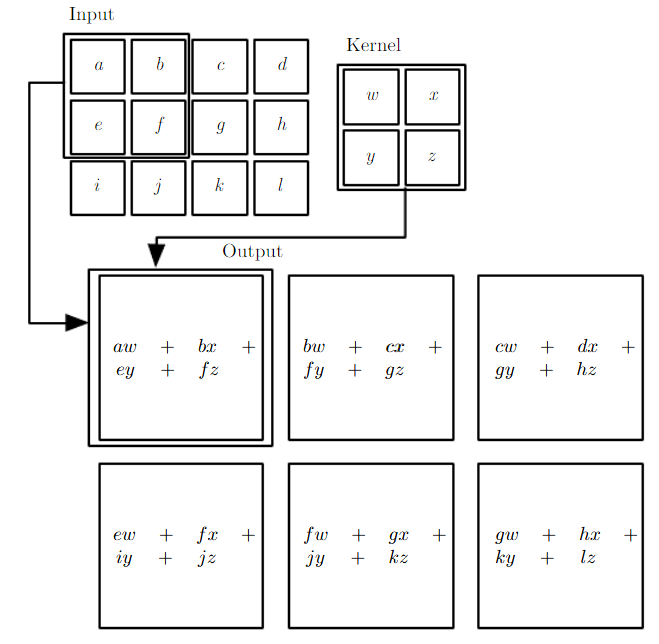
\includegraphics[width = 0.5 \textwidth]{./entities/2d_conv_example.PNG}
    \caption{An example of applying a 2d kernel on an input \cite{DL_book}.}
    \label{fig:2d_conv_example}
\end{figure}
\noindent A \textbf{convolutional layer} is a specialized kind of feedforward layer, usually used in analysis of time-series or image data. If a network has at least one convolutional layer, it is called a \textbf{Convolutional neural network (CNN)} \cite{DL_book}.
\\
\\
\noindent The convolutional layer consists of a set of \textbf{kernels}, each to be applied to the entire input vector, where each kernel is a learnable parameter matrix $k \times k$ \cite{everything}. Each kernel is applied on the input to produce a \textbf{feature map}. The kernels are applied to the input by "sliding" over the input (where the step size is called \textbf{stride}). Each $k \times k$ grid of the input is then used to compute the dot-product between the grid and each kernel, which is then placed in the corresponding feature map of each kernel, as visualized in Figure \ref{fig:2d_conv_example}. \cite{bsc_thesis}. To control the dimensions of the output, one might \textbf{pad} the sides with a constant value. Commonly, zero is used as the padding-value.
\\
\\
As seen in Figure \ref{fig:2d_conv_example}, each kernel produces a linear combination of all pixel values in a neighbourhood defined by the size of the kernel. Thus, unlike a fully-connected layer, a convolutional layer captures the high correlation between a pixel and its neighbours. Further, by limiting the size of the kernel, the network will use much fewer parameters, than if it was replaced by a fully-connected layer \cite{DL_book}.

\subsection{Recurrent Neural Networks}
\begin{figure}[htbp]
    \centering
    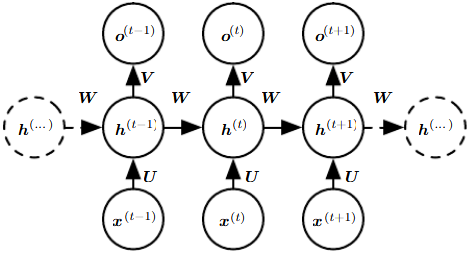
\includegraphics[width = 0.5 \textwidth]{./entities/rnn_illustration.PNG}
    \caption{An illustration of an RNN \cite{DL_book}.}
    \label{fig:rnn_illustration}
\end{figure}
\noindent \textbf{Recurrent neural networks (RNNs)} are a family of neural networks for processing sequential data. Figure \ref{fig:rnn_illustration} illustrates the general setup of such a network, which maps an input sequence of $\bm{x}$ values to a corresponding sequence of output $\bm{o}$ values. Generally, a RNN consists of three parts: (1) the input ($\bm{x}^{(i)}$), (2) the hidden state ($\bm{h}^{(i)}$), and (3) the output ($\bm{o}^{(i)}$). During inference, the model maps each input value to an output value in a sequential matter, where it first maps the first input value, then the second, then the third, and so forth. The network maps each input value to an output value by making use of the hidden state from the preceding step, where the first hidden state has to be initiallized \cite{DL_book}.

\subsubsection{Convolutional Long Short-Term Memory}
One common recurrent neural network unit is the \textbf{convolutional long short-term memory (ConvLSTM)}, which is an adaptation of the standard \textbf{long short-term memory (LSTM)} for sequences of images. Both LSTMs work by potentially stacking multiple \textbf{cells} together, such that each LSTM cell is taking in outputs of the preceding LSTM cell as its input. 
\\
\\
\noindent The idea of both LSTM cells is to create paths through time that have derivatives that neither vanish nor explode. This is done by introducing a memory cell $\mathsf{C}_t$, which accumulates state information over a long duration. This cell is accessed, written and cleared by several controlling gates. The model learns during training, when to access, write and clear this memory cell. By using the memory cell and gates to control the flow of information, the gradient will be trapped in the cell and thus be prevented from vanishing too quickly \cite{DL_book,conv_lstm}.
\\
\\
The ConvLSTM cell consists of three gates. The first gate is the input gate $\mathsf{I}_t$, which controls whether or not to accumulate the information of a new input to the cell. This gate is defined as
\begin{equation}
    \mathsf{I}_t = \sigma \left( \mathsf{W}_{xi} * \mathsf{X}_t + \mathsf{W}_{hi} * \mathsf{H}_{t - 1} + \mathsf{W}_{ci} \circ \mathsf{C}_{t - 1} + \mathsf{B}_i \right)
\end{equation}
where $\mathsf{X}_t$ is the current input image, $\mathsf{H}_{t - 1}$ is the hidden state of the previous time step, $\mathsf{C}_{t - 1}$ is the cell output of the previous time step, and $\mathsf{W}_{xi}$, $\mathsf{W}_{hi}$, $\mathsf{W}_{ci}$ and $\mathsf{B}_i$ are learnable parameters
\\
\\
The second gate is the \textbf{forget gate} unit $\mathsf{F}_t$ (at time step $t$), which controls whether or not to "forget" the status of the cell output of the previous time step. The forget gate is defined as
\begin{equation}
    \mathsf{F}_t = \sigma \left( \mathsf{W}_{xf} * \mathsf{X}_t + \mathsf{W}_{hf} * \mathsf{H}_{t - 1} + \mathsf{W}_{cf} \circ \mathsf{C}_{t - 1} + \mathsf{B}_f \right)
\end{equation}
where $\mathsf{W}_{xf}$, $\mathsf{W}_{hf}$, $\mathsf{W}_{cf}$ and $\mathsf{B}_f$ are learnable parameters.
\\
\\
The last gate is the \textbf{output gate} unit $\mathsf{O}_t$, which controls whether or not the latest cell output will be proagated to the final state $\mathsf{H}_t$. This cell is defined as
\begin{equation}
    \mathsf{O}_t = \sigma \left( \mathsf{W}_{xo} * \mathsf{X}_t + \mathsf{W}_{ho} * \mathsf{H}_{t - 1} + \mathsf{W}_{co} \circ \mathsf{C}_t + \mathsf{B}_o \right)
\end{equation}
where $\mathsf{W}_{xo}$, $\mathsf{W}_{ho}$, $\mathsf{W}_{co}$ and $\mathsf{B}_o$ are learnable parameters.
\\
\\
By combining the three gates, we get the following definition of the ConvLSTM Cell.
Let $\mathsf{X}_1, \mathsf{X}_2, ..., \mathsf{X}_t$ be a sequence of input images. Then, at each time step $t$, we compute \cite{conv_lstm}
\begin{align}
    \mathsf{I}_t &= \sigma \left( \mathsf{W}_{xi} * \mathsf{X}_t + \mathsf{W}_{hi} * \mathsf{H}_{t - 1} + \mathsf{W}_{ci} \circ \mathsf{C}_{t - 1} + \mathsf{B}_i \right) \\
    \mathsf{F}_t &= \sigma \left( \mathsf{W}_{xf} * \mathsf{X}_t + \mathsf{W}_{hf} * \mathsf{H}_{t - 1} + \mathsf{W}_{cf} \circ \mathsf{C}_{t - 1} + \mathsf{B}_f \right) \\
    \mathsf{C}_t &= \mathsf{F}_t \circ \mathsf{C}_{t - 1} + \mathsf{I}_t \circ \text{tanh} \left( \mathsf{W}_{xc} * \mathsf{X}_t + \mathsf{W}_{hc} * \mathsf{H}_{t - 1} + \mathsf{B}_c \right) \\
    \mathsf{O}_t &= \sigma \left( \mathsf{W}_{xo} * \mathsf{X}_t + \mathsf{W}_{ho} * \mathsf{H}_{t - 1} + \mathsf{W}_{co} \circ \mathsf{C}_t + \mathsf{B}_o \right) \\
    \mathsf{H}_t &= \mathsf{O}_t \circ \text{tanh}(\mathsf{C}_t)
\end{align}
For $t = 1$, both $\mathsf{H}_{t - 1}$ and $\mathsf{C}_{t - 1}$ have to be initialized \cite{conv_lstm}.

\subsubsection{Gated Recurrent Unit}


\subsection{Transformer}
\begin{figure}[htbp]
    \centering
    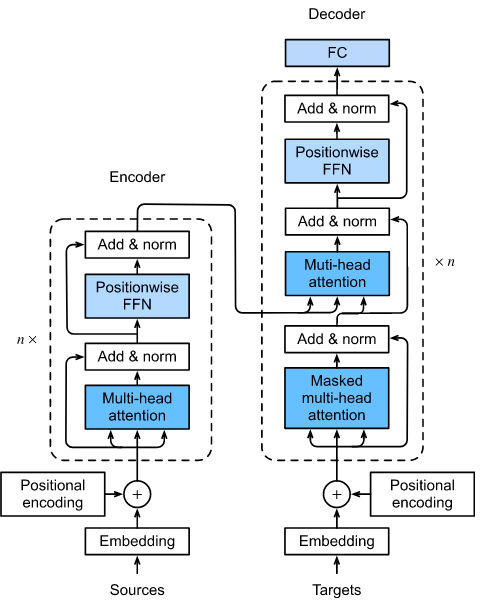
\includegraphics[width = 0.5 \textwidth]{./entities/transformer.PNG}
    \caption{An illustration of the Transformer architecture \cite{d2l}.}
    \label{fig:transformer_illustration}
\end{figure}
The sequential nature of RNNs precludes parallelization withing training examples, heavily slowing down the training of these models. Another type of model for sequential data is the \textbf{Transformer}, which eschews recurrence and instead relies on the \textbf{attention} mechanism to draw dependencies between input and output The Transformer allows for more parallelization and can reach state of the art results \cite{https://doi.org/10.48550/arxiv.1706.03762}.
\\
\\
The Transformer follow an encoder-decoder structure, where the encoder maps an input sequence $\bm{x}$ to a sequence of continuous representations $\bm{z}$. The decoder then uses $\bm{z}$ to generate an output sequence $\bm{y}$, one element at a time. At each step the model consumes the previously generated output element as additional input when generating the next output \cite{https://doi.org/10.48550/arxiv.1706.03762}. Figure \ref{fig:transormer_illustration} illustrates the overall Transformer architecture.

\subsubsection{Attention}
bla bla bla
\\
\\
\textbf{Scaled Dot-Product Attention:} bla bla bla 
\\
\\
\textbf{Multi-Head Attention: }  bla bla bla

\subsubsection{Encoder}
The encoder consists of $N$ identical layers, where each layer consists of two sub-layers. The first sub-layer is a \textbf{multi-head} \textbf{self-attention} mechanism, and the second sub-layer is a position-wise fully connected feed-forward network. Around each sub-layer is a \textbf{residual connection}, which is followed by a round of \textbf{layer normalization} \cite{https://doi.org/10.48550/arxiv.1706.03762}.

\subsubsection{Decoder}
The decoder also consists of $N$ identical layers. In addition to the two sub-layers in each encoder layer, the decoder also consists of a third sub-layer, which performs multi-head attention over the output of the encoder stack. Also here, is residual connections used around each of the sub-layers, followed by layer normalization. To ensure, that the predicitons for position $i$ only depends on the known outputs at positions less than $i$, the self-attention sub-layer in the decoder stack is modified \cite{https://doi.org/10.48550/arxiv.1706.03762}.

\subsection{Training a Neural Network}
\subsubsection{Activation function}
\subsubsection{multi-head}
\subsubsection{self-attention}
\subsubsection{attention}
\subsubsection{residual connection}
\subsubsection{layer normalization}
\label{subsubsec:activation_func}

\end{document}